%\documentclass[aps,prl,twocolumn,showpacs,superscriptaddress,groupedaddress]{revtex4}  % for review and submission
%\documentclass[aps,preprint,showpacs,superscriptaddress,groupedaddress]{revtex4}  % for double-spaced preprint
%\documentclass[aps,prl,floatfix,twocolumn,10pt]{revtex4-1}  % for review and submission
%\documentclass[aps,prl,preprint]{revtex4-1}  % for double-spaced preprint
\documentclass[aip,apl,amsmath,amssymb,floatfix,reprint,a4paper]{revtex4-1}

%% Packages
\usepackage{graphicx}  %figures
\usepackage{subfigure} %subfigures
\usepackage{amssymb}   %math
\usepackage{upgreek}   %non-italic greek letters
\usepackage[utf8]{inputenc} %Umlaute

%% hyphenation settings
\hyphenation{ALPGEN}
\hyphenation{EVTGEN}
\hyphenation{PYTHIA}

%% New commands
\newcommand{\unit}[1]{\ensuremath{\, \mathrm{#1}}}
\newcommand{\msub}[1]{\ensuremath{\textnormal{\begin{tiny}#1\end{tiny}}}}

%% ----------------------------------------------------------------------------------------------------------------
\begin{document}

\title{X-ray phase-contrast imaging at 100~keV}

\author{T.~Thüring}
  \affiliation{Paul Scherrer Institut, Villigen PSI, Switzerland}
  \affiliation{Institute for Biomedical Engineering, Swiss Federal Institute of Technology, Zurich, Switzerland}
\author{M.~Abis}
  \affiliation{Paul Scherrer Institut, Villigen PSI, Switzerland}
  \affiliation{Institute for Biomedical Engineering, Swiss Federal Institute of Technology, Zurich, Switzerland}
\author{Z.~Wang}
  \affiliation{Paul Scherrer Institut, Villigen PSI, Switzerland}
\author{C.~David}
  \affiliation{Paul Scherrer Institut, Villigen PSI, Switzerland}
\author{M.~Stampanoni}
  \affiliation{Paul Scherrer Institut, Villigen PSI, Switzerland}
  \affiliation{Institute for Biomedical Engineering, Swiss Federal Institute of Technology, Zurich, Switzerland}

\date{\today}


%% ----------------------------------------------------------------------------------------------------------------
\begin{abstract}
Phase contrast imaging with X-rays is an exciting modality that reveals new insights into material properties by providing access to a complementary physical contrast mechanism. Phase sensitive imaging in the high energy range of hard X-rays, i.e. above 60 keV is still largely unexplored, as the currently availabe methods are technically limited. We demonstrate a novel approach, which enables the access to the entire diagnostic energy range of X-rays for phase contast as well as dark field contrast imaging on laboratory systems with low brilliance X-ray sources. A phase contrast technique at such high energies is of particularly high scientific and industrial interest as it would vastly expand the range of applications, for instance, by the examination of materials of high density or thickness. The approach exploits the principles of differential phase contrast imaging and employs a new technique for diffraction grating manufacturing, which is compatible to any X-ray energy in the diagnostic range. Firstly, the approach breaks the current limits of achievable grating aspect ratios, which has been the key issue in the past. Secondly, it solves the intrinsic reduction of the field of view, which occurs for such high grating aspect ratios. An imaging arrangement has been set up, which allows to acquire phase- and dark-field-contrast images at $100 \unit{keV}$ for the first time. This successful step forward to access the high diagnositc energy range will pave the road for the transfer of phase contrast imaging into fields where high energies are required, such as medical CT, chip failure analysis or homeland security.
%The examination in phase contrast of dense materials, such as metals, has not been feasible so far due to the high absorption and scattering cross sections in the lower energy range.
%requires  is the electron density  provides direct access to electron densityovercomes the limitation in the achievable contrast in objects with low absorbing materials and  
\end{abstract}

\maketitle

%%%%%%%%%%%%%%%%%%%%%%%%%%%%%%%%%%%%%%%%%%%%%%%%%%%%%%%%%%%%%%%%%%%%%%%%
% Body of manuscript
%%%%%%%%%%%%%%%%%%%%%%%%%%%%%%%%%%%%%%%%%%%%%%%%%%%%%%%%%%%%%%%%%%%%%%%%
X-ray radiography and computed tomography (CT) are nowadays standard imaging techniques in materials and life science for the non-destructive examination of samples. The physical contrast mechanism relies on the attenuation of X-rays in an object through the photo-electric effect or Compton scattering, whereas two materials can be distinguished due to their different attenuation properties. Apart from attenuation, the wave and particle nature of X-rays reveal two further physical interaction mechanisms that occur if an object is exposed to X-rays.

Regarding the wave properties, a transition from one medium into another causes a change in the wave's phase velocity and thus in a net change of the output phase (a phase shift) downstream of the object. Since no detection device is able to measure a phase shift directly, advanced techniques are necessary to obtain access to this signal.

Regarding the particle properties of X-rays, photons are randomly scattered on fine structures in the material. Depending on the imaging system (geometry and energy), wide angle and small angle scattering are considered as typical sources of noise in conventional X-ray images. For the special type of scattering which occurs exclusively in forward direction and under ultra small angles (order of nano radiants), the particles usually remain within the area of a detector pixel. This effect is not recorded by absorption images and cannot directly be detected with standard techniques.

The main interest in the detectability of those additional interaction mechanisms is the fact that attenuation, phase shift and scattering are physically complementary interaction mechanisms, in the sense that their occurrence is mutually independent. This gives rise to hypothesize that the complementary interaction mechanisms may eventually yield complementary image contrasts.

A huge effort has been invested in the past into the discovery of techniques which are sensitive to phase shift or scattering events. Since currently available phase contrast techniques rely on secondary physical effects, such as interference, and thus typically on optical hardware (e.g. crystals, gratings), they vary a lot in terms of sensitivity, practical applicability or achievable resolution. The vast majority of the methods, including crystal analyzer based \cite{Davis1995,Chapman1997} or interferometric \cite{Bonse1965,Momose1996} methods rely on X-ray beams of high spatial and temporal coherence, available only at synchrotrons. Techniques with a high degree of spectral acceptance are the in-line phase contrast method \cite{Snigirev1995,Wilkins1996,Cloetens1996} and Talbot interferometry \cite{Cloetens1997,David2002,Momose2003a}. Regarding the acceptance of X-ray beams with low temporal and spatial coherence (i.e. beams of low-brilliance X-ray source), Talbot-Lau interferometry \cite{Pfeiffer2006} and coded apertures \cite{Munro2012} are currently the only compatible techniques.

Phase contrast techniques are nowadays widely available on synchrotrons, whereas only a few are applicable on compact imaging arrangements with conventional X-ray tubes. Up to now, none of the methods is compatible to the higher energy range of hard X-rays ($>50 \unit{keV}$). Therefore, imaging tasks requiring phase contrast at such high energies have so far been infeasible. Prominent examples are for instance medical imaging tasks such as chest or abdominal radiography or CT, which require energies up to $150 \unit{keV}$. Due to the low spatial coherence of typical X-ray sources in this energy range, in-line phase contrast methods are not promising. For the most promising technique, which is Talbot-Lau interferometry, grating fabrication is limited to X-ray energies up to approx. $50 \unit{keV}$ where the grating aspect ratio is the technical limiting factor. The aspect ratio, given by
\begin{equation}
 \textnormal{AR} = \frac{2h}{p},
\end{equation}
where $p$ is the grating period and $h$ the grating structure height, cannot be aribtrarily high, as grating structures tend to collapse or to deform due to capillary forces. For a given setup distance and for $p \propto 1/\sqrt{E}$ and $h \propto E^3$, it can be shown that $\textnormal{AR} \propto E^{7/2}$. While for $25 \unit{keV}$, an aspect ratio for the absorption grating of around $\textnormal{AR}=30$ is necessary for a reasonable length of the experimental arrangement, it would have to be at least 128 for $100 \unit{keV}$. Moreover, when using a polychromatic spectrum, photons above the design energy should also be efficiently attenuated by the gratings to guarantee their contribution to the signal, which requires even higher aspect ratios. The maximum aspect ratio, which has not significantly improved in the past few years, is $\textnormal{AR} \approx 60$, whereas such high values are often even beyond the limit and come at the expense of a poor grating quality and performance.

Here, we introduce a novel approach, which is based on Talbot-Lau interferometry and allows phase contrast and dark field imaging with low brilliance X-ray tubes at arbitrarily high energies. The approach is based on a new grating design, aiming at the edge-on illumination of gratings. Edge-on illumination, as opposed to face-on illumination, exploits the dimension along the grating lines to form a high aspect ratio of the structures in beam direction. The effective structure height of the grating is then determined by the grating dimension along the grating lines, which essentially allows arbitrarily high aspect ratios. FIG.~\ref{Fig:schematic} illustrates the edge-on illumination approach.
\begin{figure} [ht]
  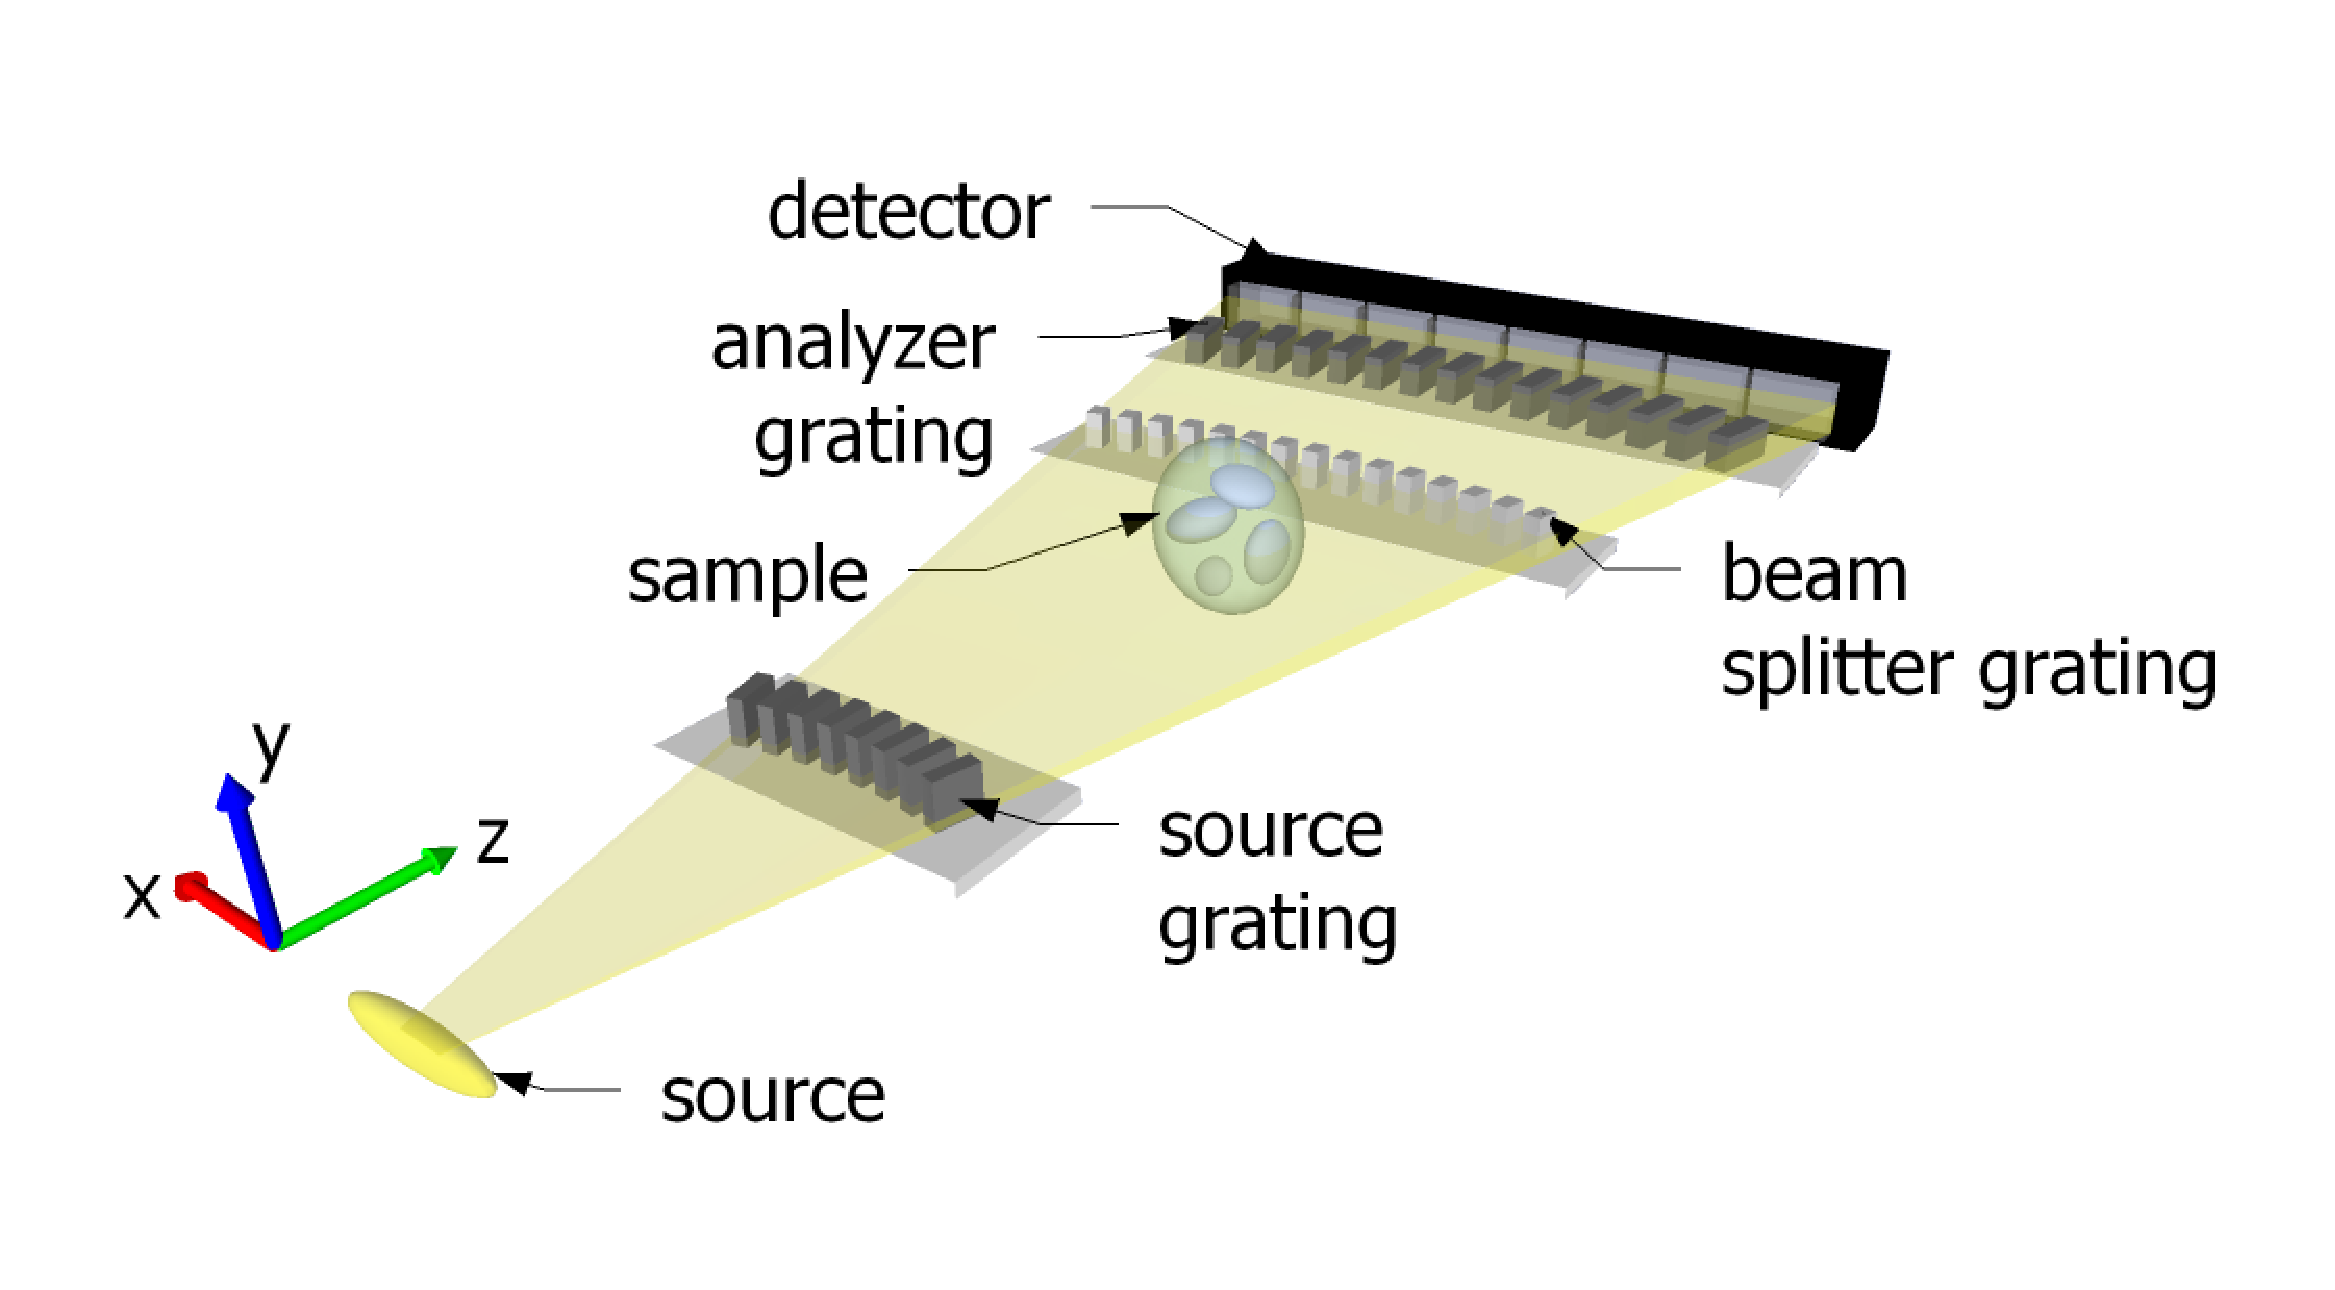
\includegraphics[width = \linewidth]{figures/figure1.eps}
  \caption{Schematic of a grating interferometer for high X-ray energies in edge-on illumination mode. The aspect ratio is defined by the ratio of the travelling distance along the grating lines and the period and can be arbitrarily long. In order to avoid a reduction of the field of view, the grating structures are aligned on an arc.}
  \label{Fig:schematic}
\end{figure}

Increasing the effective aspect ratio of the gratings typically leads to a reduction of the field of view due to the change of the grating transmission function at high incident angles, which has also been identified by using a glancing angle of the gratings between zero and $90$ degrees \cite{Stutman2012a}. In order to overcome this problem with edge-on illuminated gratings, the grating lines are aligned on an arc with a radius equal to the distance to the source.

The combination of edge-on illumination and the circularly curved structures allows design energies in the entire diagnostic energy range of X-rays. The arbitrary aspect ratio only comes at the expense of a limited field of view in the vertical dimension of the image plane, which is, depending on the detector, typically a few pixels. However, radiographic 2D images can still be acquired in sample scanning mode without increasing dose. Similarly, for tomographic images, the approach allows single slice CT or full 3D imaging in scanning mode.

Grating design and fabrication is non-standard and involves a complex mask design, as shown in FIG.~\ref{Fig:grating_mask}. Each grating resides on a silicon chip and has its specific structure length and curvature. For the present experiments, a symmetric interferometer with a grating period of $p = 2.8 \unit{\upmu m}$ for all gratings has been used. The design energy is $100 \unit{keV}$ and the beam splitter grating periodically shifts the phase by zero and $\pi$ at this energy. Using gold as the phase shifting material, this requires a structure length of $h_1 = 19.8 \unit{\upmu m}$. The analyzer grating is an absorption mask for sensing slight changes of the interference pattern generated by the beam splitter. With a structure length of $h_2 = 800 \unit{\upmu m}$, this grating has an aspect ratio of $2h/p \approx 570$ and thus sufficiently attenuates X-rays up to energies of around $160 \unit{keV}$. Beam splitter- and analyzer grating are separated at the first fractional Talbot order \cite{Weitkamp2005}, resulting in an inter-grating distance of $158 \unit{mm}$. The source grating splits the relatively large focal spot ($\sim 1 \unit{mm}$ into an array of individually coherent, but mutually incoherent sources \cite{Pfeiffer2006}. It is also made of gold structures with a structure length of $h_0 = h_2 = 800 \unit{\upmu m}$.
\begin{figure} [ht]
  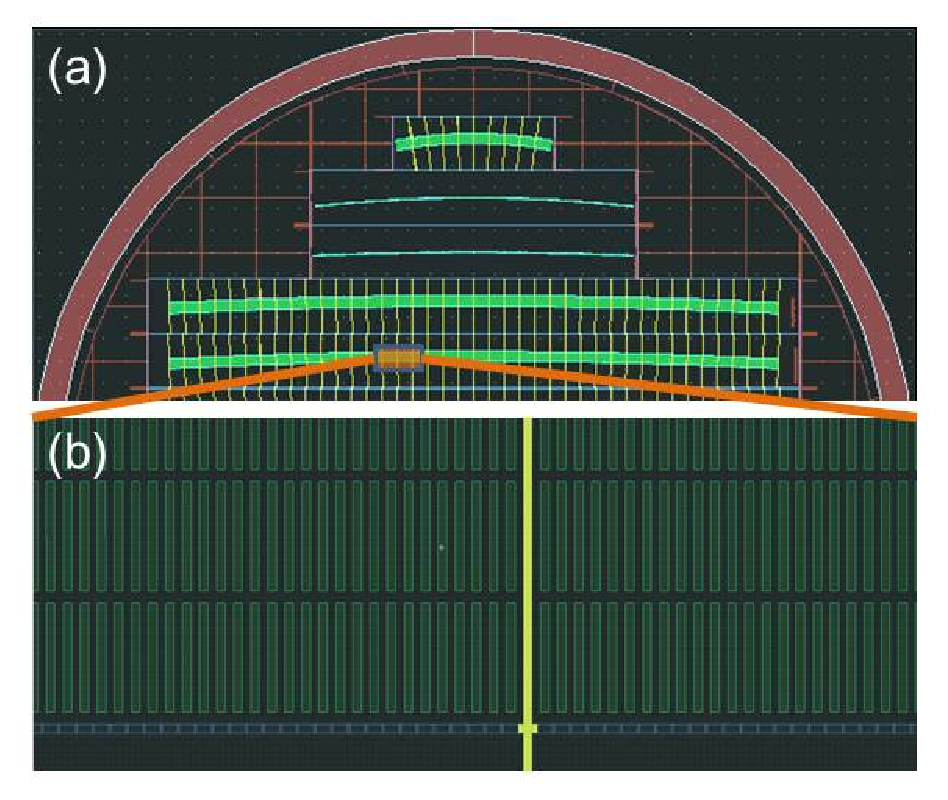
\includegraphics[width = \linewidth]{figures/grating_mask.eps}
  \caption{Grating design mask for the edge-on illumination approach. (a) Top part of the 4 inch wafer, showing five grating chips; one source grating, two beam splitter gratings and two analyzer gratings (from top to bottom). The gratings have different curvatures which are specific to the grating interferometer geometry. (b) Zoom into the grating structures, contain interrupting bridges used for stabilizing the grating structures in the LIGA process.}
  \label{Fig:grating_mask}
\end{figure}

Due to the high spectral acceptance \cite{Weitkamp2005,Thuering2013c} of the interferometer ($50 \unit{keV}$ to $>160 \unit{keV}$) and the high attenuation efficiencies of the source- and analyzer gratings (<10\% up to $160 \unit{keV}$), the voltage of the X-ray source was set to the maximum of $160 \unit{kV}$. With a grating structure height of approx. $100 \unit{\upmu m}$, the field of view in the vertical direction is limited to one detector pixel row. In the horizontal direction, the field of view is limited by the grating size and the geometric magnification of the sample, yielding a maximum of $30 \unit{mm}$. In addition to the standard components (source, camera, interferometer), two optical slits, one in front of the source grating, the other in front of the camera, were required for the collimation of the beam in the vertical direction. X-rays which are not travelling through all of the gratings do not contribute to the signal and are attenuated by the slits.

Fig. 3 shows a radiographic image of a metal screw in all three contrast modes, acquired with the $100 \unit{keV}$ setup. The images were acquired in scanning mode, using a step size of $100 \unit{\upmu m}$. The number of phase steps was 24 and the exposure time was 15 seconds per step. Grating interferometry at such a high diagnostic energy allows to examine more dense materials such as metals in phase contrast mode. At lower energies, the phase shifts of such materials would be too large and wrap over multiple periods of the analyzer grating.



Fig. 4 shows another example of a radiographic scan of an electronic chip. The scan parameters were the same as for the previous example. Several resistors and an integrated circuit are located on a different layer on the chip. In the attenuation based projection image, the soldering points of the integrated circuit are hardly visibible underneath the resistors. In the phase image, they can clearly be identified. Furthermore, the phase image reveals variations in the shape of these soldering points. This illustrates how the differential nature of the phase contrast signal could potentially be used to identify flaws in multi-layered electronic chips, which might remain undetected on the absorption image.



Edge-on illuminated grating interferometry breaks the current limitation to the low diagnostic energy range for X-ray phase contrast imaging with conventional X-ray sources. Compact geometries for design energies well above 100 keV can be realized for the examination of dense materials which would be intransparent at lower energies of currently used phase contrast techniques. The approach is not limited to X-ray imaging, it can also be applied to other grating based imaging modalities (e.g., with neutrons \cite{Grunzweig2008}) where high aspect ratios are necessary.

\section*{Methods}
Edge-on illuminated gratings were manufactured by Micro Works GmbH, Germany, using a LIGA process \cite{Kenntner2010}. Each grating resides on a $5 \times 60 \unit{mm^2}$ silicon chip and several grating chips are fabricated on a single 4 inch silicon wafer. The experimental arrangement for a design energy at 100 keV is a symmetric Talbot-Lau interferometer with a grating period of $p = 2.8 \unit{\upmu m}$ for all gratings. The distance from the source grating to the analyzer grating is $32 \unit{cm}$ and the source grating is positioned $23 \unit{cm}$ away from the source. The number of phase steps for one projection was 24 \cite{Weitkamp2005} and the exposure time for the images was 15 seconds per phase steps.

The X-ray source is a COMET MXR-160HP/11 X-ray tube with a maximum output voltage of $160 \unit{kV}$. In the experiment, it was set to the maximum voltage. The focal spot size is approximately $1 \unit{mm}$. The detector is a CCD camera from Finger Lakes Instruments. A cesium iodide (CsI:Ti) scintillator of $600 \unit{\upmu m}$ thickness converts the X-rays to visible light and is coupled with an optical lens projecting the image onto the CCD. The effective pixel size is $80 \unit{\upmu m}$. The widths of the collimating slits are $25 \unit{\upmu m}$ and $100 \unit{\upmu m}$, respectively.

\section*{Acknowledgements}
We thank Gordan Mikuljan from Paul Scherrer Institute, Switzerland, for his work on the mechanical design, Joachim Schulz and Marco Walter from Micro Works GmbH, Germany, for the competent support on grating design issues, Christian Kottler and Vincent Revol from Centre Suisse d'Electronique et de Microtechnique (CSEM), Switzerland for the fruitful discussions on grating interferometer design.



\bibliography{library.bib}
\bibliographystyle{apsrev4-1}

\end{document}